\section{Styringsenhed}\label{sec:Styringsenhed:design}
\subsection{ADC}

Da signalprocesseringen også kan foregå på PSoC 5LP er denne platform et oplagt valg til også at designe styringsenhedens ADC'er i. Herved kan analog til digital konvertering og processering integreres i ét modul. Der ses i figur\tbr \ref{fig} et flowdiagram over den tiltænkte virkemåde for ADC og DSP i styringsenheden. 

Til designet af denne enhed er der som inspiration brugt et bredt udvalg af applikationsnoter fra Cypress Semiconductor som har udviklet PSoC 5LP. Den pågældende er af familien CY8C58xx. Opsætningen og implementeringen af ADC og DSP blokken er gjort i PSoC Creator 4.3. 

Delta Sigma ADC komponenten på PSoC kan enten konfigueres ved firmware eller ved et grafisk interface i PSoC Creator 4.3. Her er det grafiske interface brugt, og i det følgende vil designovervejelserne dokumenteres.

\subsubsection{Analog interfaces}
For at få bedst mulig interface til mikrofonforstærker og filter er der på baggrund af applikationsnoten AN58304, s. 3 \tbr REFERENCE  ... valgt port [P0:7] som indgang til ADC'en, da denne er en af de foreskrevne analoge porte med bedst performance. 

\subsubsection{Input range}
\begin{figure}
    \centering
    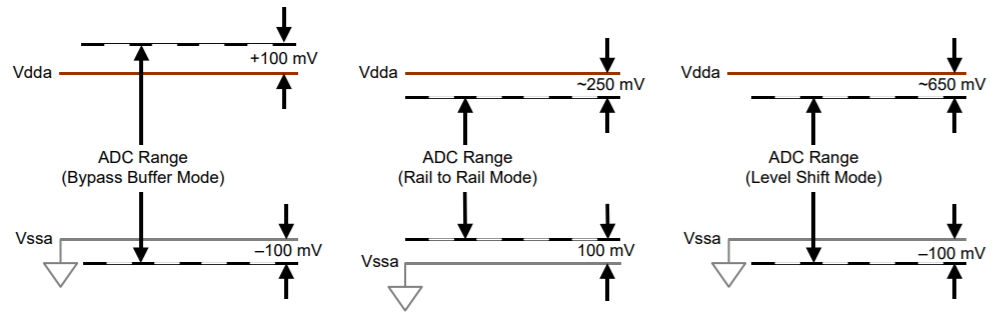
\includegraphics{figs/Design/Styringsenhed/inputrange.PNG}
    \caption{Forskellige input modes for Delta Sigma ADC}
    \label{fig:ADC_inputrange}
\end{figure}
For at få så meget headroom og derved opløsning som muligt, konfigueres ADC'en til (i princippet) rail to rail operation. Men ved denne konfiguration i PSoC aktiveres en buffer på indgangen for at give mulighed for at forstærke indganssignalet. Dette fravælges (bufferen bypasses), for at opnå størst muligt headroom og derved opløsning, se Figur \ref{fig:ADC_inputrange}. Hertil opnås den højest mulige indgangsimpedans,  da anvendelsen af denne buffer er på bekostning af indgangsimpedansen.\tbr REFERENCE TIL DELTA SIGMA ADC, s. 12. Hvis der herved opstår problemer med overstyring af ADC'en, kan der konfigureres til rail-to-rail med buffer gain på 1. 

\subsubsection{Input mode}
\subsubsection{Referencespændinger}
PSoC 5LP har interne referencespændinger med en tolerance på +- 0.1\%. \tbr Reference til datablad for PSoC, side 94.



\subsubsection{Interrupt, polling, DMA}





\subsection{DSP blokken}

\begin{functionDescription}
    {uint8 DoFFT(uint8* inputArray, uint16* FFTResultPtr)}
    {func:DoFFT}
    {Funktionen udregner 128 FFT koefficienter, der efterbefølgende behandles som et styringssignal. }
    {inputArray: Pointer til den samplede ADC data\newline
    FFTResultPTR: Pointer til den de udregnede FFT koefficienter}
    {Ingen}
\end{functionDescription}